\documentclass[11pt]{article}

\usepackage{amsmath,amssymb,mathtools}
\usepackage[margin=1in]{geometry}
\usepackage{enumitem}
\usepackage{xcolor}
\usepackage{microtype}
\usepackage{graphicx}
\usepackage{tikz,float}
\usepackage{subcaption}
\usepackage{amsthm}
\usepackage{hyperref}
\usepackage{array}
\usepackage{pgfplots}

\usetikzlibrary{shapes.geometric, arrows.meta, positioning, calc, decorations.markings}
\tikzset{
	block/.style={rectangle, draw, text width=6em, text centered, rounded corners, minimum height=10mm},
	sum/.style={circle, draw, node distance=1.5cm},
	line/.style={draw, -{Stealth[length=2.5mm, width=1.5mm]}}
}

\usepgfplotslibrary{groupplots}
\pgfplotsset{compat=1.18}

\pgfplotsset{
	myaxes/.style={
		axis lines=middle,
		axis line style={-latex},
		grid=major,
		grid style={gray!15},
		minor grid style={gray!35},
		xlabel style={at={(ticklabel* cs:1)}, anchor=north west},
		ylabel style={at={(ticklabel* cs:1)}, anchor=south east},
		every axis plot/.append style={thick}
	},
	myplotstyle/.style={
		width=14cm,
		height=7cm,
		axis lines=middle,
		axis line style={-Stealth},
		grid=both,
		minor tick num=1,
		major grid style={draw=gray!30},
		minor grid style={draw=gray!15},
		tick label style={font=\small, fill=white, inner sep=1.5pt},
		xlabel={$t$},
		ylabel={$x(t)$},
		xlabel style={anchor=north east, font=\small},
		ylabel style={anchor=south east, font=\small},
		samples=401,
	}
}

\newtheoremstyle{mynote}
{6pt}      % Space above
{6pt}      % Space below
{}          % Body font (normal, not italic)
{}          % Indent amount
{\bfseries} % Theorem head font
{.}         % Punctuation after theorem head
{.5em}      % Space after theorem head
{}          % Theorem head spec
\theoremstyle{mynote}
\newtheorem{definition}{Definition}
\newtheorem{proposition}{Proposition}
\newtheorem{example}{Example}
\newtheorem{remark}{Remark}
\newtheorem{theorem}{Theorem}
\newtheorem{corollary}{Corollary}

\newcommand{\T}{\mathcal{T}}
\newcommand{\R}{\mathbb{R}}
\newcommand{\Z}{\mathbb{Z}}
\newcommand{\C}{\mathbb{C}}
\newcommand{\conv}{\ast}
\newcommand{\dt}{\,\dd t}
\newcommand{\dd}{\mathrm{d}}
\newcommand{\imp}{\delta}
\newcommand{\sinc}[1]{\frac{\sin(\pi #1)}{\pi #1}}


\DeclareMathOperator{\rect}{rect}
\DeclareMathOperator{\Ev}{Ev}
\DeclareMathOperator{\Od}{Od}
\DeclareMathOperator{\sgn}{sgn}
\DeclareMathOperator{\step}{u}
\DeclareMathOperator{\tri}{tri}

\usetikzlibrary{angles,quotes,arrows.meta}
\pgfmathdeclarefunction{tri}{2}{%
	\pgfmathparse{2*abs(mod(#1, #2)/(0.5*#2) - 1) - 1}%
}

\begin{document}
	% Reset figure counter for this lecture
	\renewcommand{\thefigure}{2.\arabic{figure}}
	
	% --- TITLE BLOCK ---
	\thispagestyle{empty}
	\noindent
	\begin{tabular*}{\textwidth}{l @{\extracolsep{\fill}} r}
		\textbf{Signals and Systems} & \textbf{Lecture 2} \\
		\textit{Dr. Ghandi Manasra and Ahmed Rabei} & \textit{Fall 2025} \\
	\end{tabular*}
	\hrule
	\vspace{0.4cm}
	\begin{center}
		\Large\textbf{Lecture 2: Elementary Signals and Signal Properties}
	\end{center}
	\vspace{0.4cm}
	
\section*{Reference}
	Oppenheim \& Willsky, \textit{Signals and Systems}, Chapter 1, Sections 1.2.2 -- 1.4

	\section*{Review of Lecture 1}
	\begin{itemize}[noitemsep]
		\item CT and DT signals defined
		\item Time-domain transformations learned
		\item Audio signal examples
		\item Energy and power concepts
	\end{itemize}
	
	\section*{2.1 Periodic Signals}
	\subsection*{Continuous-Time (CT) Periodic Signals}
	\begin{definition}
		A CT signal $x(t)$ is \textbf{periodic} if there exists a constant $T > 0$ such that
		\[
		x(t) = x(t + T), \quad \forall t \in \R.
		\]
	\end{definition}
	
	\begin{itemize}[noitemsep]
		\item The \textbf{fundamental period} $T_0$ is the smallest such positive value of $T$.
		\item If $T_0$ is the fundamental period, then $mT_0$ is also a period for any integer $m$.
		\item The \textbf{fundamental frequency} is given by:
		\[
		f_0 = \frac{1}{T_0} \text{ (in Hz)}, \quad \omega_0 = 2\pi f_0 = \frac{2\pi}{T_0} \text{ (in rad/s)}.
		\]
	\end{itemize}
	
	% --- PLOT: Periodic CT Triangular Wave ---
	\begin{figure}[H]
		\centering
		\begin{figure}[H]
	\centering
	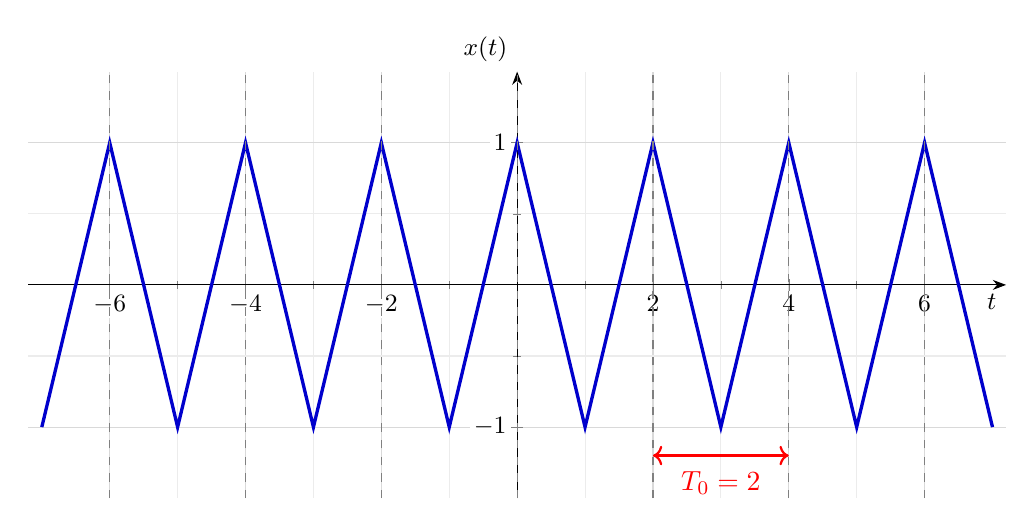
\begin{tikzpicture}
		\begin{axis}[
			myplotstyle,
			xmin=-7.2, xmax=7.2,
			ymin=-1.5, ymax=1.5,
			xtick={-6,-4,-2,0,2,4,6},
			ytick={-1,0,1},
			]
			% Triangular wave
			\addplot[blue!80!black, very thick] coordinates {
				(-7,-1) (-6,1) (-5,-1) (-4,1) (-3,-1) (-2,1) (-1,-1)
				(0,1) (1,-1) (2,1) (3,-1) (4,1) (5,-1) (6,1) (7,-1)
			};
			
			% Vertical dashed lines (use pgfplots loop helper)
			\pgfplotsinvokeforeach{-6,-4,-2,0,2,4,6}{
				\draw[gray, dashed] (axis cs:#1,-1.5) -- (axis cs:#1,1.5);
			}
			
			% Period annotation
			\draw[<->, red, thick]
			(axis cs:2,-1.2) -- (axis cs:4,-1.2)
			node[midway, below=2pt] {$T_0=2$};
		\end{axis}
	\end{tikzpicture}
\end{figure}

		\caption{Periodic continuous-time triangular wave.}
		\label{fig:ct_periodic_triangular}
	\end{figure}
	
	\begin{example}
		Show that \(x(t) = A\cos(\omega_0 t + \theta)\) has a fundamental period of 
		\[
		T_0 = \frac{2\pi}{|\omega_0|}.
		\]
	\end{example}
	
	\paragraph{Sum of Periodic CT Signals:} A sum of two periodic signals, \(x(t) = x_1(t) + x_2(t)\) with fundamental periods \(T_1\) and \(T_2\), is periodic if and only if the ratio of their periods is a rational number:
	\[
	\frac{T_1}{T_2} = \frac{m}{n}, \quad \text{where } m, n \in \Z^+.
	\]
	The fundamental period is then 
	\[
	T_0 = nT_1 = mT_2,
	\]
	where \(m,n\) are the smallest such integers. This means \(T_0\) is the smallest time when the first signal has completed \(m\) full cycles and the second signal has completed \(n\) full cycles simultaneously, marking the moment they "align" perfectly and the combined signal repeats.
	
	% --- PLOT: Sum of two periodic CT signals ---
	\begin{figure}[H]
		\centering
		\begin{figure}[H]
	\centering
	\begin{subfigure}[b]{\textwidth}
		\centering
		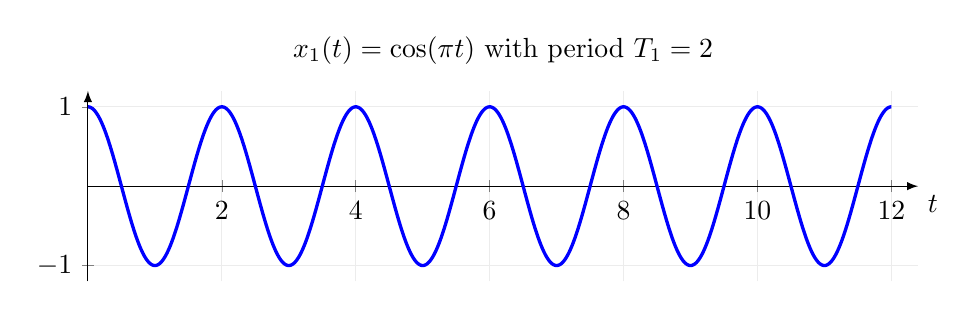
\begin{tikzpicture}
			\begin{axis}[
				width=\linewidth, height=4cm,
				myaxes,
				title={$x_1(t)=\cos(\pi t)$ with period $T_1=2$},
				xlabel={$t$}, xmin=0, xmax=12.4,
				ymin=-1.2, ymax=1.2,
				samples=1201,
				smooth
				]
				\addplot[blue, very thick, domain=0:12] {cos(deg(pi*x))};
			\end{axis}
		\end{tikzpicture}
	\end{subfigure}
	\\
	\begin{subfigure}[b]{\textwidth}
		\centering
		\begin{tikzpicture}
			\begin{axis}[
				width=\linewidth, height=4cm,
				myaxes,
				title={$x_2(t)$ is a triangular wave with period $T_2=3$},
				xlabel={$t$}, xmin=0, xmax=12.4,
				ymin=-1.2, ymax=1.2,
				samples=1201,
				smooth
				]
				\addplot[red, very thick, domain=0:12] {tri(x,3)};
			\end{axis}
		\end{tikzpicture}
	\end{subfigure}
	\\
	\begin{subfigure}[b]{\textwidth}
		\centering
		\begin{tikzpicture}
			\begin{axis}[
				width=\linewidth, height=5cm,
				myaxes,
				title={Sum: $x(t)=x_1(t)+x_2(t)$, with period $T_0=\mathrm{lcm}(2,3)=6$},
				xlabel={$t$}, xmin=0, xmax=12.4,
				ymin=-2.2, ymax=2.2,
				samples=1801,
				smooth
				]
				\addplot[purple, very thick, domain=0:12] {cos(deg(pi*x)) + tri(x,3)};
				% Period annotation
				\draw[<->, red, thick] (axis cs:0,-1.6) -- node[below] {$T_0=6$} (axis cs:6,-1.6);
			\end{axis}
		\end{tikzpicture}
	\end{subfigure}
\end{figure}
		\caption{Sum of two periodic continuous-time signals.}
		\label{fig:sum_ct_periodic}
	\end{figure}
	% --- PLOT: Sum of two signals resulting in an aperiodic one ---
	\vspace*{\fill}
	\begin{figure}[H]
		\centering
		\begin{figure}[H]
    \centering
	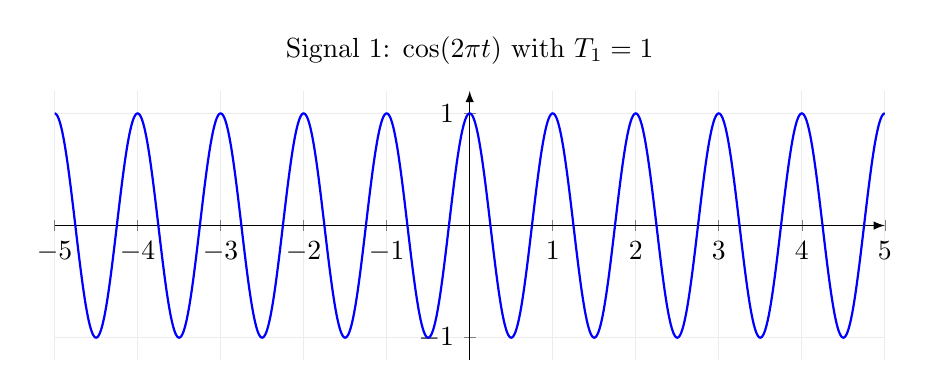
\begin{tikzpicture}
		\begin{axis}[
			width=\textwidth, height=5cm, myaxes,
			title={Signal 1: \(\cos(2\pi t)\) with \(T_1=1\)},
			xmin=-5, xmax=5, ymin=-1.2, ymax=1.2,
			samples=1001, smooth
			]
			\addplot[blue, thick] {cos(deg(2*pi*x))};
		\end{axis}
	\end{tikzpicture}
	\vspace{1em}
	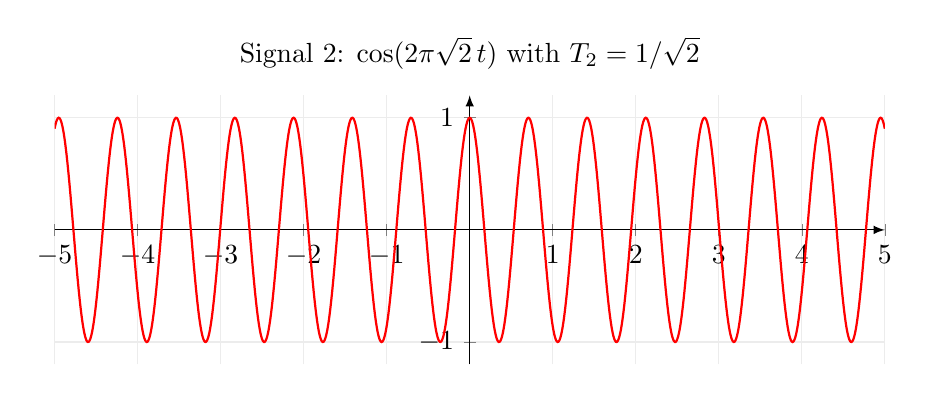
\begin{tikzpicture}
		\begin{axis}[
			width=\textwidth, height=5cm, myaxes,
			title={Signal 2: \(\cos(2\pi\sqrt{2}\,t)\) with \(T_2=1/\sqrt{2}\)},
			xmin=-5, xmax=5, ymin=-1.2, ymax=1.2,
			samples=1001, smooth
			]
			\addplot[red, thick] {cos(deg(2*pi*sqrt(2)*x))};
		\end{axis}
	\end{tikzpicture}
	\vspace{1em}
	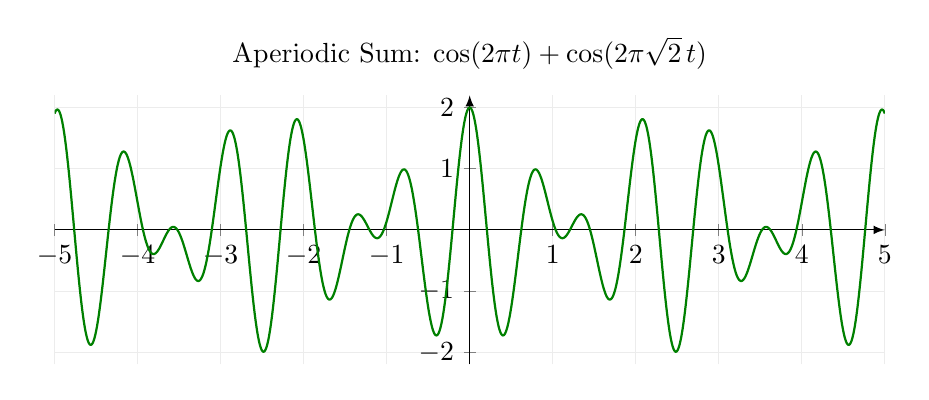
\begin{tikzpicture}
		\begin{axis}[
			width=\textwidth, height=5cm, myaxes,
			title={Aperiodic Sum: \(\cos(2\pi t)+\cos(2\pi\sqrt{2}\,t)\)},
			xmin=-5, xmax=5, ymin=-2.2, ymax=2.2,
			samples=2001, smooth
			]
			\addplot[green!50!black, thick] {cos(deg(2*pi*x)) + cos(deg(2*pi*sqrt(2)*x))};
		\end{axis}
	\end{tikzpicture}
\end{figure}
		\caption{Sum of periodic signals creating aperiodic result.}
		\label{fig:sum_ct_aperiodic}
	\end{figure}
	\vspace*{\fill}
	\newpage
	\subsection*{Discrete-Time (DT) Periodic Signals}
	\begin{definition}
		A DT signal $x[n]$ is \textbf{periodic} if there exists an integer $N > 0$ such that
		\[
		x[n] = x[n+N], \quad \forall n \in \Z.
		\]
	\end{definition}
	
	\begin{itemize}[noitemsep]
		\item The \textbf{fundamental period} $N_0$ is the smallest such positive integer.
		\item If $N_0$ is a period, then $mN_0$ is also a period for any integer $m$.
		\item The fundamental angular frequency is \(\omega_0 = \frac{2\pi}{N_0}\) (in rad/sample).
	\end{itemize}
	
	% --- PLOT: Periodic DT Triangular Wave ---
	\begin{figure}[H]
		\centering
		\begin{figure}[H]
	\centering
    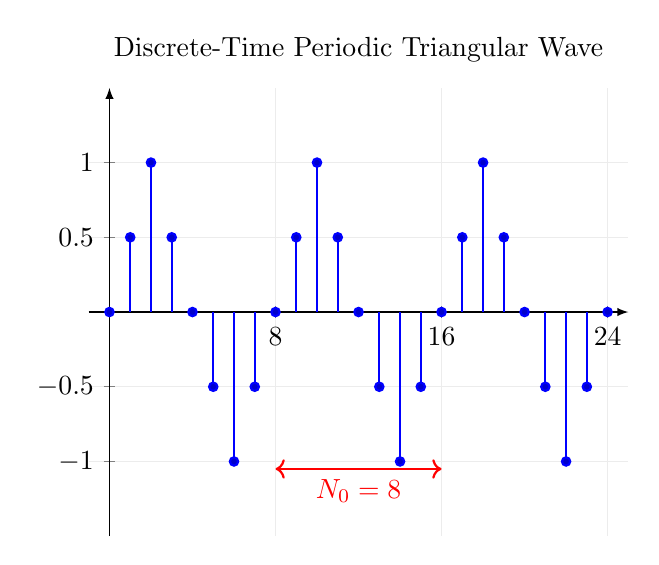
\begin{tikzpicture}
      \begin{axis}[
        myaxes,
        title={Discrete-Time Periodic Triangular Wave},
        xmin=-1, xmax=25,
        ymin=-1.5, ymax=1.5,
        xtick={0,8,16,24},
        ytick={-1,-0.5,0,0.5,1},
        enlargelimits=false
      ]
        \addplot+[ycomb, blue, thick, mark=*, mark size=1.5pt] table {
          x y
          0 0
          1 0.5
          2 1
          3 0.5
          4 0
          5 -0.5
          6 -1
          7 -0.5
          8 0
          9 0.5
          10 1
          11 0.5
          12 0
          13 -0.5
          14 -1
          15 -0.5
          16 0
          17 0.5
          18 1
          19 0.5
          20 0
          21 -0.5
          22 -1
          23 -0.5
          24 0
        };
        \draw[<->, red, thick] 
          (axis cs:8,-1.05) -- (axis cs:16,-1.05)
          node[midway, below] {$N_0=8$};
      \end{axis}
	\end{tikzpicture}
\end{figure}
		\caption{Periodic discrete-time triangular wave.}
		\label{fig:dt_periodic_triangular}
	\end{figure}
	
	\paragraph{Sum of Periodic DT Signals:}
	If \(x_1[n]\) has period \(N_1\) and \(x_2[n]\) has period \(N_2\), their sum \(x[n] = x_1[n] + x_2[n]\) is periodic with period \(N_0\) given by 
	\[
	N_0 = \operatorname{lcm}(N_1, N_2) = \frac{N_1 N_2}{\operatorname{gcd}(N_1, N_2)}.
	\]
	For \(x[n]\) to be periodic, both \(x_1[n]\) and \(x_2[n]\) must complete an integer number of their respective periods simultaneously. The smallest such interval is the fundamental period \(N_0\) of the sum. 
	\newpage
	\begin{example}
		\begin{itemize}[noitemsep]
			\item \(N_1=6, N_2=9 \implies N_0 = \operatorname{lcm}(6,9) = 18.\)
			\item \(N_1=8, N_2=12 \implies N_0 = \operatorname{lcm}(8,12) = 24.\)
		\end{itemize}
	\end{example}
	
	% --- PLOT: Sum of two periodic DT signals ---
	\begin{figure}[H]
		\centering
		\begin{figure}[H]
	\centering
	\begin{subfigure}{\textwidth}
		\centering
		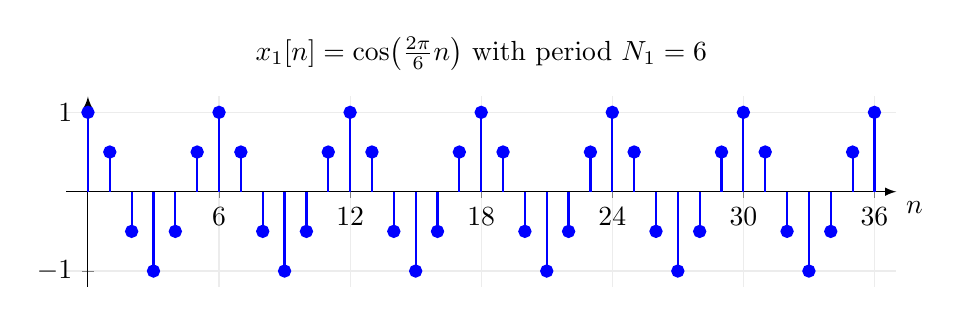
\begin{tikzpicture}
			\begin{axis}[
				width=\linewidth, height=4cm, myaxes, ycomb,
				title={\(x_1[n]=\cos\!\left(\tfrac{2\pi}{6}n\right)\) with period \(N_1=6\)},
				xlabel={\(n\)}, xmin=-1, xmax=37, ymin=-1.2, ymax=1.2,
				xtick={0, 6, 12, 18, 24, 30, 36}
				]
				\addplot[samples at={0,...,36}, blue, thick, mark=*] {cos(360/6*x)};
			\end{axis}
		\end{tikzpicture}
	\end{subfigure}
	\vspace{0.5cm}
	\begin{subfigure}{\textwidth}
		\centering
		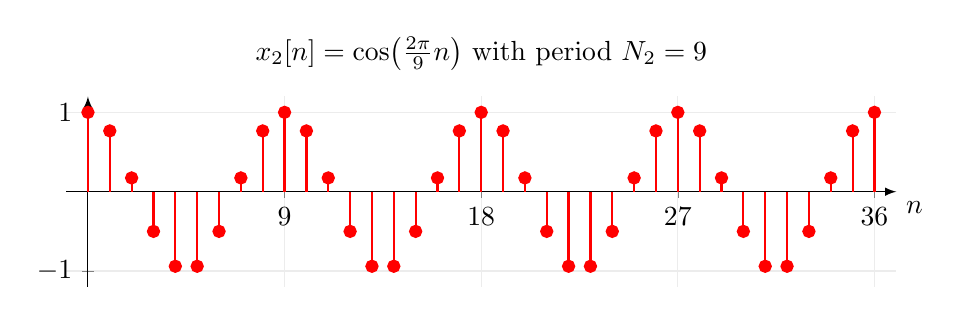
\begin{tikzpicture}
			\begin{axis}[
				width=\linewidth, height=4cm, myaxes, ycomb,
				title={\(x_2[n]=\cos\!\left(\tfrac{2\pi}{9}n\right)\) with period \(N_2=9\)},
				xlabel={\(n\)}, xmin=-1, xmax=37, ymin=-1.2, ymax=1.2,
				xtick={0, 9, 18, 27, 36}
				]
				\addplot[samples at={0,...,36}, red, thick, mark=*] {cos(360/9*x)};
			\end{axis}
		\end{tikzpicture}
	\end{subfigure}
	\vspace{0.5cm}
	\begin{subfigure}{\textwidth}
		\centering
		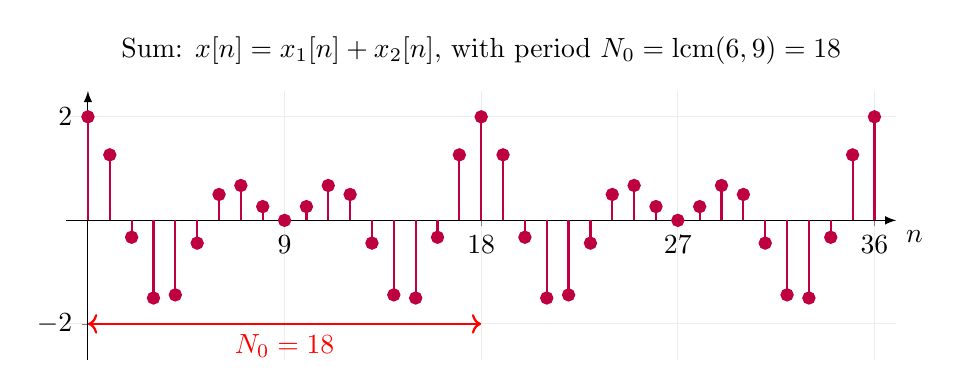
\begin{tikzpicture}
			\begin{axis}[
				width=\linewidth, height=5cm, myaxes, ycomb,
				title={Sum: \(x[n]=x_1[n]+x_2[n]\), with period \(N_0=\operatorname{lcm}(6,9)=18\)},
				xlabel={\(n\)}, xmin=-1, xmax=37, ymin=-2.7, ymax=2.5,
				xtick={0, 9, 18, 27, 36}
				]
				\addplot[samples at={0,...,36}, purple, thick, mark=*] {cos(360/6*x) + cos(360/9*x)};
				\draw[<->, red, thick] (axis cs:0, -2.0) -- (axis cs:18, -2.0)
				node[midway, below] {\(N_0=18\)};
			\end{axis}
		\end{tikzpicture}
	\end{subfigure}
\end{figure}
		\caption{Sum of two periodic discrete-time signals.}
		\label{fig:sum_dt_periodic}
	\end{figure}
	
	\hrulefill
	
	\subsection*{Average Power of Periodic Signals}
	Periodic signals are classified as \textbf{power signals}. Their average power can be computed over one fundamental period (\(T_0\) or \(N_0\)) as follows:
	\begin{itemize}[noitemsep]
		\item CT average power:
		\[
		P_{\text{ave}} = \frac{1}{T_0} \int_{t_0} |x(t)|^2 \, \dt.
		\]
		\item DT average power:
		\[
		P_{\text{ave}} = \frac{1}{N_0} \sum_{n=\langle N_0\rangle} |x[n]|^2.
		\]
	\end{itemize}
	
	\pagebreak
	
	\section*{2.2 Even and Odd Signals}
	A signal can be classified based on its symmetry with respect to the time origin.
	
	\begin{definition}
		\textbf{Even signal:} Symmetric about the vertical axis.
		\[
		x(-t) = x(t) \quad \text{(CT)}, \quad x[-n] = x[n] \quad \text{(DT)}.
		\]
	\end{definition}
	
	% --- PLOT: Even Signals ---
	\begin{figure}[H]
		\centering
		\begin{figure}[H]
	\centering
	\begin{subfigure}{0.48\textwidth}
		\centering
		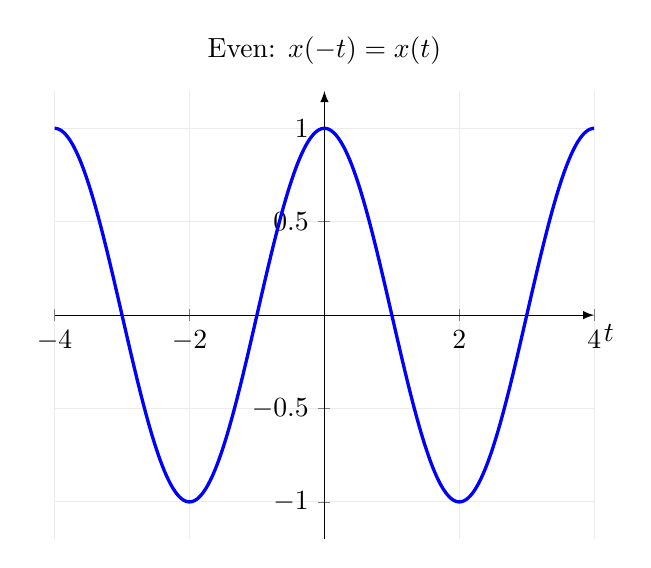
\begin{tikzpicture}
			\begin{axis}[myaxes, title={Even: \(x(-t)=x(t)\)},
				xlabel={$t$}, ylabel={},
				xmin=-4, xmax=4, ymin=-1.2, ymax=1.2]
				\addplot[domain=-4:4, samples=400, blue, very thick] {cos(90*x)};
			\end{axis}
		\end{tikzpicture}
	\end{subfigure}
	\hfill
	\begin{subfigure}{0.48\textwidth}
		\centering
		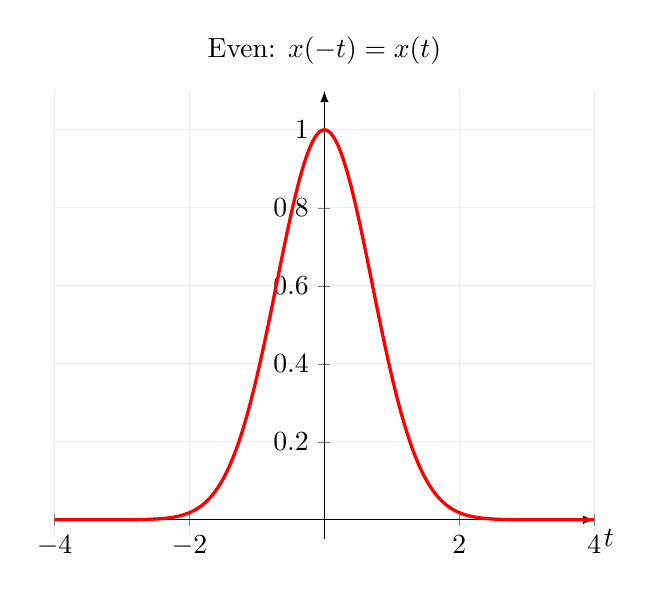
\begin{tikzpicture}
			\begin{axis}[myaxes, title={Even: \(x(-t)=x(t)\)},
				xlabel={$t$}, ylabel={},
				xmin=-4, xmax=4, ymin=-0.05, ymax=1.1]
				\addplot[domain=-4:4, samples=400, red, very thick] {exp(-x^2)};
			\end{axis}
		\end{tikzpicture}
	\end{subfigure}
\end{figure}
		\caption{Even signal symmetry examples.}
		\label{fig:even_signals}
	\end{figure}
	
	\begin{definition}
		\textbf{Odd signal:} Symmetric about the origin.
		\[
		x(-t) = -x(t) \quad \text{(CT)}, \quad x[-n] = -x[n] \quad \text{(DT)}.
		\]
	\end{definition}
	
	% --- PLOT: Odd Signals ---
	\begin{figure}[H]
		\centering
		\begin{figure}[H]
	\centering
	\begin{subfigure}{0.48\textwidth}
		\centering
		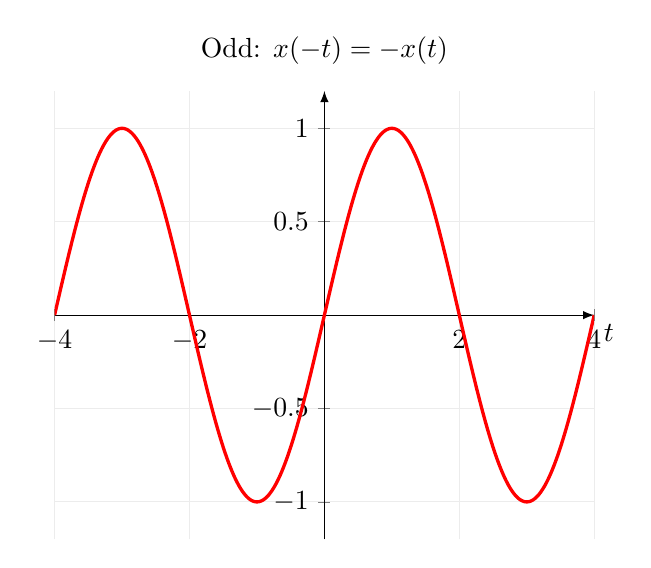
\begin{tikzpicture}
			\begin{axis}[myaxes, title={Odd: \(x(-t)=-x(t)\)},
				xlabel={$t$}, ylabel={},
				xmin=-4, xmax=4, ymin=-1.2, ymax=1.2]
				\addplot[domain=-4:4, samples=400, red, very thick] {sin(90*x)};
			\end{axis}
		\end{tikzpicture}
	\end{subfigure}
	\hfill
	\begin{subfigure}{0.48\textwidth}
		\centering
		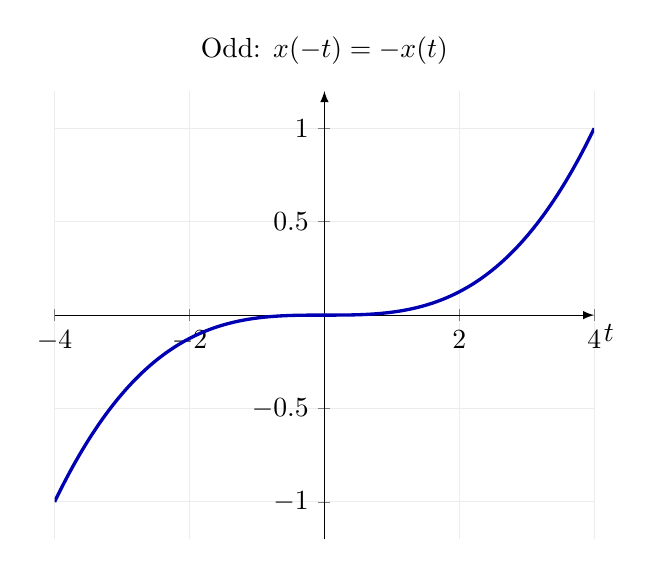
\begin{tikzpicture}
			\begin{axis}[myaxes, title={Odd: \(x(-t)=-x(t)\)},
				xlabel={$t$}, ylabel={},
				xmin=-4, xmax=4, ymin=-1.2, ymax=1.2]
				\addplot[domain=-4:4, samples=400, very thick, color=blue!70!black] {x^3/64};
			\end{axis}
		\end{tikzpicture}
	\end{subfigure}
\end{figure}
		\caption{Odd signal symmetry examples.}
		\label{fig:odd_signals}
	\end{figure}
	
	\begin{proposition}
		Any signal can be decomposed into the sum of an even part and an odd part:
		\[
		x(t) = x_e(t) + x_o(t),
		\]
		where the even and odd components are given by:
		\[
		x_e(t) = \frac{1}{2} \left( x(t) + x(-t) \right), \quad x_o(t) = \frac{1}{2} \left( x(t) - x(-t) \right).
		\]
		The same decomposition applies to DT signals by replacing \(t\) by \(n\).
	\end{proposition}
	
	% --- PLOT: Even and Odd Decomposition ---
	\begin{figure}[H]
		\centering
		\begin{figure}[H]
	\centering
	\begin{subfigure}{\textwidth}
		\centering
		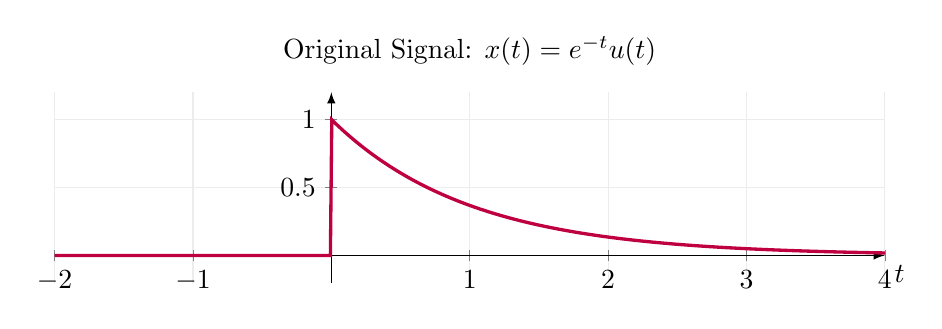
\begin{tikzpicture}
			\begin{axis}[width=\linewidth, height=4cm, myaxes,
				title={Original Signal: \(x(t)=e^{-t}u(t)\)},
				xlabel={$t$}, xmin=-2, xmax=4, ymin=-0.2, ymax=1.2]
				\addplot[domain=-2:4, samples=600, purple, very thick]
				{(x>=0) ? exp(-x) : 0};
			\end{axis}
		\end{tikzpicture}
	\end{subfigure}
	\vspace{0.3cm}
	\begin{subfigure}{\textwidth}
		\centering
		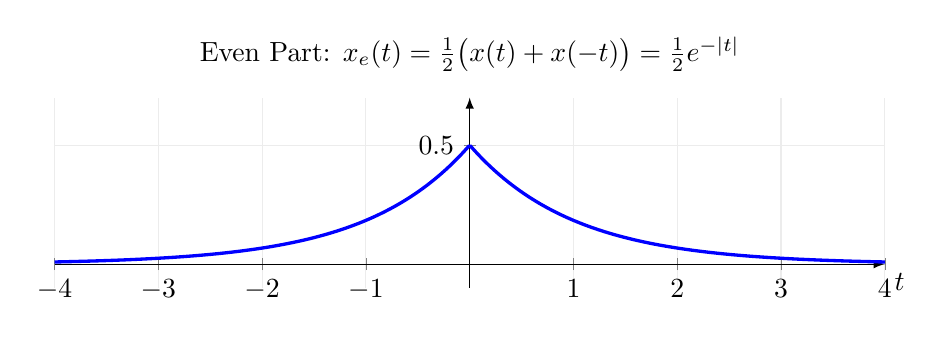
\begin{tikzpicture}
			\begin{axis}[width=\linewidth, height=4cm, myaxes,
				title={Even Part: \(x_e(t)=\tfrac{1}{2}\big(x(t)+x(-t)\big)=\tfrac{1}{2}e^{-|t|}\)},
				xlabel={$t$}, xmin=-4, xmax=4, ymin=-0.1, ymax=0.7,
				ytick distance=0.5]
				\addplot[domain=-4:4, samples=400, blue, very thick] {0.5*exp(-abs(x))};
			\end{axis}
		\end{tikzpicture}
	\end{subfigure}
	\vspace{0.3cm}
	\begin{subfigure}{\textwidth}
		\centering
		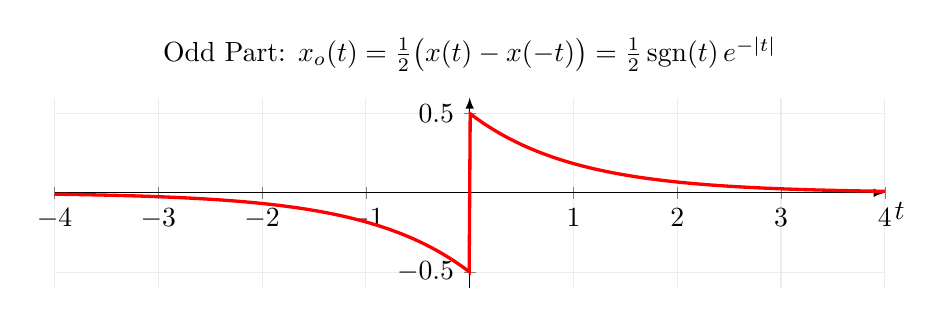
\begin{tikzpicture}
			\begin{axis}[width=\linewidth, height=4cm, myaxes,
				title={Odd Part: \(x_o(t)=\tfrac{1}{2}\big(x(t)-x(-t)\big)=\tfrac{1}{2}\operatorname{sgn}(t)\,e^{-|t|}\)},
				xlabel={$t$}, xmin=-4, xmax=4, ymin=-0.6, ymax=0.6]
				\addplot[domain=-4:4, samples=800, red, very thick]
				{0.5*((x>=0 ? exp(-x) : 0) - (x<=0 ? exp(x) : 0))};
			\end{axis}
		\end{tikzpicture}
	\end{subfigure}
\end{figure}
		\caption{Signal decomposition into even and odd parts.}
		\label{fig:even_odd_decomposition}
	\end{figure}
	
	\paragraph{Energy of Even/Odd Parts:} Because the even and odd components of a signal are orthogonal, the total energy of a signal is the sum of the energies of its even and odd parts:
	\[
	\int_{-\infty}^\infty |x(t)|^2 \dt = \int_{-\infty}^\infty |x_e(t)|^2 \dt + \int_{-\infty}^\infty |x_o(t)|^2 \dt.
	\]
	The same applies for DT signals by replacing integration with summation and t with n.
	
	\pagebreak
	
	\section*{2.3 Exponential and Sinusoidal Signals}
	\subsection*{Continuous-Time (CT) Exponentials}
	The general form is:
	\[
	x(t) = C e^{a t}, \quad \text{where } a, C \in \C.
	\]
	
	% --- PLOT: Real and Complex Exponentials ---
\begin{figure}[H]
	\centering
	\resizebox{0.8\textwidth}{!}{
	\begin{subfigure}{0.45\textwidth}
		\centering
		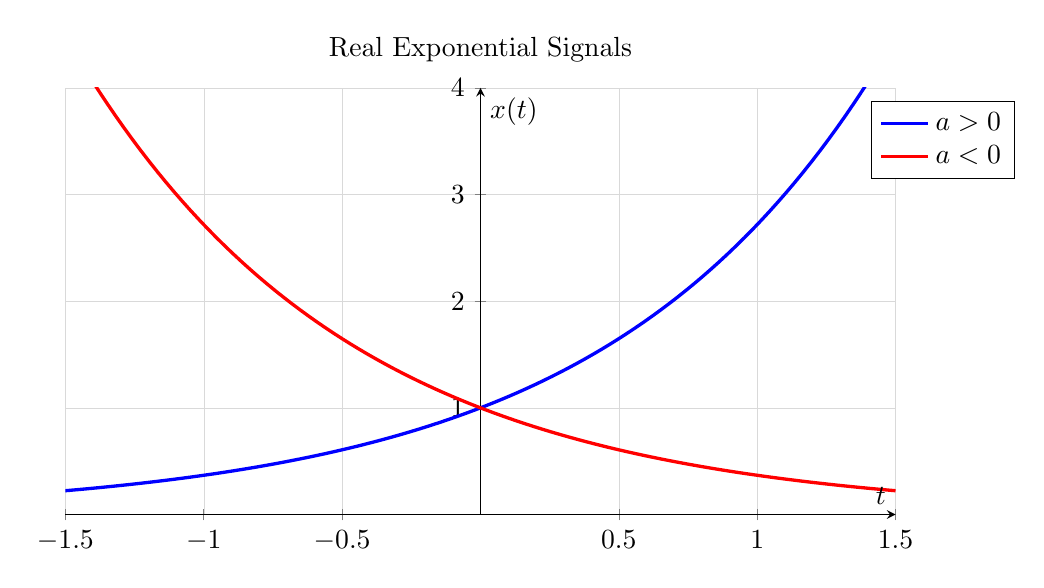
\begin{tikzpicture}
			\begin{axis}[
				width=\linewidth,
				height=7cm,
				title={Real Exponential Signals},
				xlabel={$t$},
				ylabel={$x(t)$},
				axis lines=middle,
				xmin=-1.5, xmax=1.5,
				ymin=0, ymax=4,
				ytick={1,2,3,4},
				grid=major,
				grid style={line width=.1pt, draw=gray!30},
				legend style={
					at={(0.97, 0.97)},
					anchor=north west,
					legend cell align={left}
				},
				no marks,
				]
				\addplot[blue, very thick, domain=-1.5:1.5, samples=100] {exp(x)};
				\addlegendentry{$a>0$}
				
				\addplot[red, very thick, domain=-1.5:1.5, samples=100] {exp(-x)};
				\addlegendentry{$a<0$}
			\end{axis}
		\end{tikzpicture}
		\caption{Real exponential signals.}
		\label{fig:real_exp}
	\end{subfigure}
	\hfill
	% --- Second Subfigure: Complex Exponential ---
	\begin{subfigure}{0.5\textwidth}
		\centering
		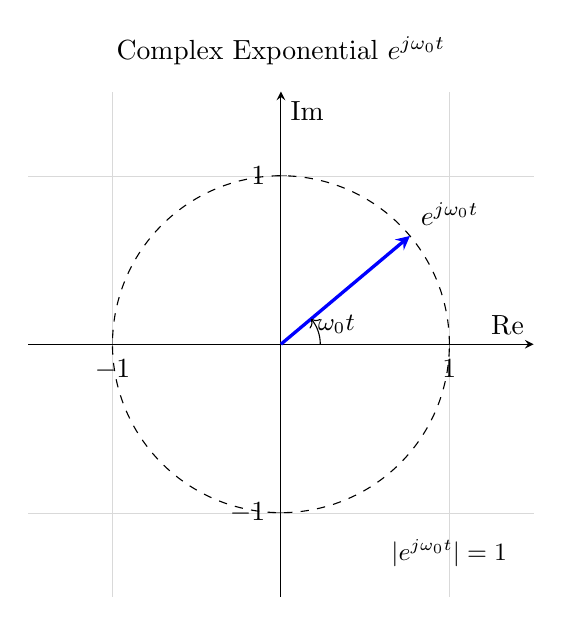
\begin{tikzpicture}
			\begin{axis}[
				width=\linewidth,
				height=8cm,
				title={Complex Exponential $e^{j\omega_0 t}$},
				xlabel={$\text{Re}$},
				ylabel={$\text{Im}$},
				axis equal image,
				axis lines=middle,
				xmin=-1.5, xmax=1.5,
				ymin=-1.5, ymax=1.5,
				xtick={-1,1},
				ytick={-1,1},
				grid=major,
				grid style={line width=.1pt, draw=gray!30},
				]
				% Draw the unit circle
				\addplot[black, dashed, domain=0:360, samples=361, no marks] ({cos(x)}, {sin(x)});
				
				% Define the angle and coordinates for the vector
				\pgfmathsetmacro{\myangle}{40}
				\coordinate (O) at (axis cs:0,0);
				\coordinate (P) at (axis cs:{cos(\myangle)},{sin(\myangle)});
				\coordinate (X) at (axis cs:1,0);
				
				% Draw the phasor (vector)
				\draw[-stealth, blue, very thick] (O) -- (P) node[above right, black] {$e^{j\omega_0 t}$};
				
				% Draw and label the angle
				\pic [draw, ->, "$\omega_0 t$", angle eccentricity=1.5, font=\small] {angle = X--O--P};
				
				% Label the magnitude
				\node[anchor=north east, font=\small] at (axis cs:1.4, -1.1) {$|e^{j\omega_0 t}|=1$};
			\end{axis}
		\end{tikzpicture}
		\caption{Complex exponential signal.}
		\label{fig:complex_exp}
	\end{subfigure}
	\label{fig:exp_signals}}
	\caption{Visualization of real and complex exponential signals.}
	\label{fig:ct_exponentials}
\end{figure}
	
	\begin{itemize}[noitemsep]
		\item \textbf{Real Exponent ($a, C \in \R$):}
		\begin{itemize}[noitemsep]
			\item If \(a > 0\), the signal grows exponentially.
			\item If \(a < 0\), the signal decays exponentially.
		\end{itemize}
		\item \textbf{Complex Exponent ($a = j \omega_0$):} The signal \(x(t) = e^{j \omega_0 t}\) is periodic. Using Euler's relation:
		\[
		x(t) = e^{j \omega_0 t} = \cos(\omega_0 t) + j \sin(\omega_0 t).
		\]
		It represents a vector of unit length rotating in the complex plane at angular frequency \(\omega_0\). Its fundamental period is
		\[
		T_0 = \frac{2\pi}{|\omega_0|}.
		\]
		\item The higher \(|\omega_0|\), the faster the vector spins, resulting in faster oscillations in the real and imaginary parts.
	\end{itemize}
	
	\subsection*{Continuous-Time (CT) Sinusoids}
	\[
	x(t) = A \cos(\omega_0 t + \theta) = \Re \left\{ A e^{j(\omega_0 t + \theta)} \right\}.
	\]
	This shows that sinusoids are projections of rotating complex exponentials onto the real axis.
	
	The fundamental frequency \(f_0\) in Hertz (cycles per second) and the fundamental period \(T_0\) are related to \(\omega_0\) as:
	\[
	f_0 = \frac{\omega_0}{2\pi}, \quad T_0 = \frac{1}{f_0} = \frac{2\pi}{\omega_0}.
	\]
	
	\subsection*{Discrete-Time (DT) Exponentials}
	The general form is:
	\[
	x[n] = C \alpha^n.
	\]
	
	% --- PLOT: DT Exponentials ---
	\begin{figure}[H]
		\centering
			\centering
	\begin{subfigure}{0.48\textwidth}
		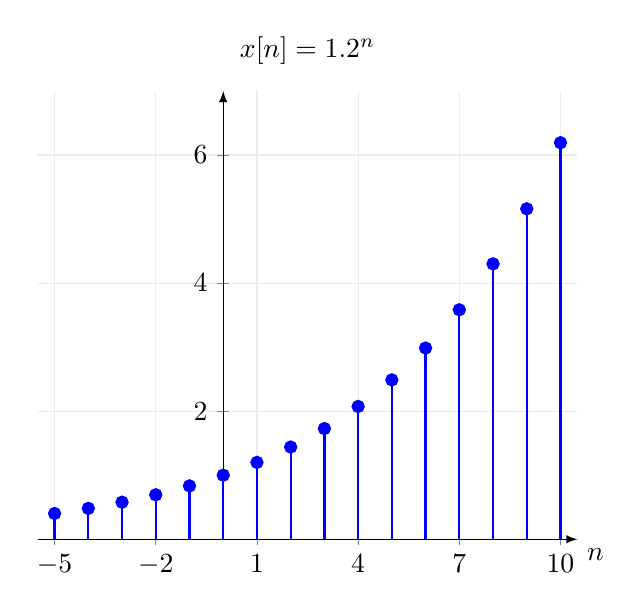
\begin{tikzpicture}
			\begin{axis}[
				myaxes, title={\(x[n]=1.2^n\)},
				xlabel={\(n\)}, ylabel={},
				xmin=-5.5, xmax=10.5, ymin=0, ymax=7,
				xtick={-5,-2,1,4,7,10}
				]
				\addplot[ycomb, blue, thick, mark=* , samples at={-5,...,10}] {1.2^x};
			\end{axis}
		\end{tikzpicture}
	\end{subfigure}
	\hfill
	\begin{subfigure}{0.48\textwidth}
		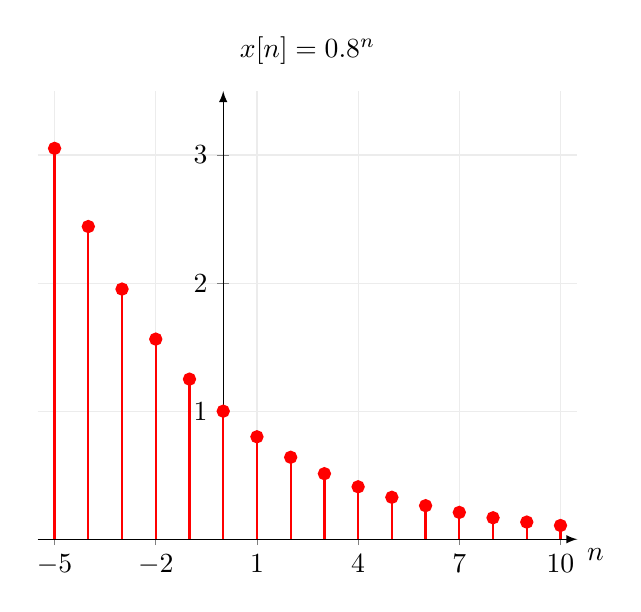
\begin{tikzpicture}
			\begin{axis}[
				myaxes, title={\(x[n]=0.8^n\)},
				xlabel={\(n\)}, ylabel={},
				xmin=-5.5, xmax=10.5, ymin=0, ymax=3.5,
				xtick={-5,-2,1,4,7,10}
				]
				\addplot[ycomb, red, thick, mark=* , samples at={-5,...,10}] {0.8^x};
			\end{axis}
		\end{tikzpicture}
	\end{subfigure}
	
	\vspace{1em}
	
	\begin{subfigure}{0.48\textwidth}
		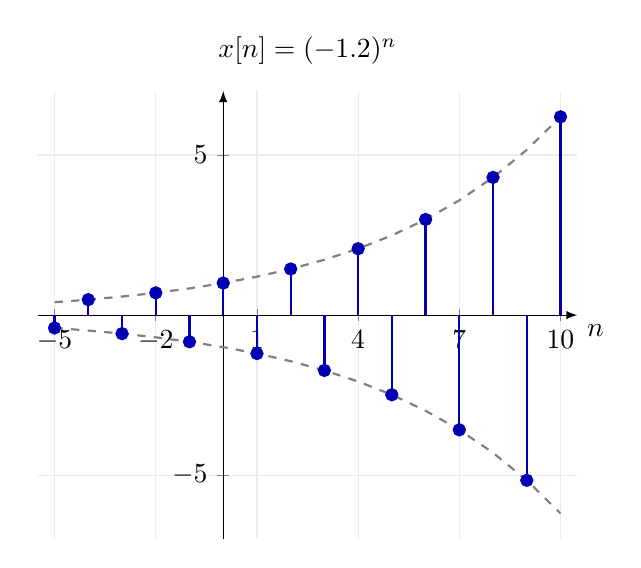
\begin{tikzpicture}
			\begin{axis}[
				myaxes, title={\(x[n]=(-1.2)^n\)},
				xlabel={\(n\)}, ylabel={},
				xmin=-5.5, xmax=10.5, ymin=-7, ymax=7,
				xtick={-5,-2,1,4,7,10}
				]
				\addplot[ycomb, blue!70!black, thick, mark=* , samples at={-5,...,10}] {(1.2^x)*cos(180*x)};
				\addplot[gray, dashed, samples at={-5,...,10}] { 1.2^x};
				\addplot[gray, dashed, samples at={-5,...,10}] {-1.2^x};
			\end{axis}
		\end{tikzpicture}
	\end{subfigure}
	\hfill
	\begin{subfigure}{0.48\textwidth}
		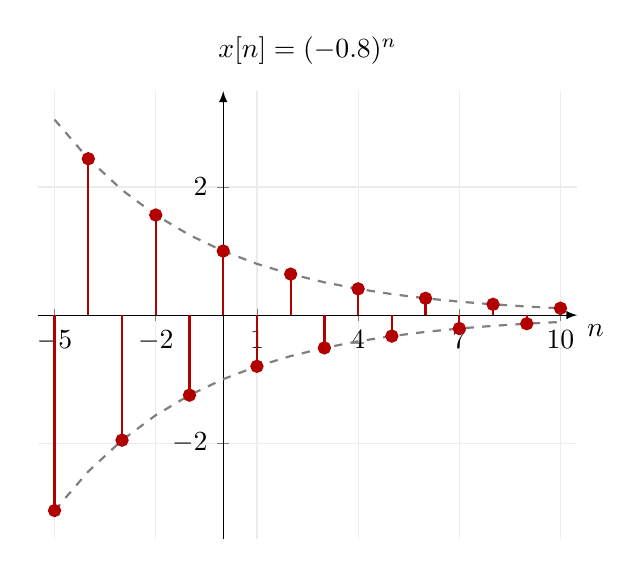
\begin{tikzpicture}
			\begin{axis}[
				myaxes, title={\(x[n]=(-0.8)^n\)},
				xlabel={\(n\)}, ylabel={},
				xmin=-5.5, xmax=10.5, ymin=-3.5, ymax=3.5,
				xtick={-5,-2,1,4,7,10}
				]
				\addplot[ycomb, red!70!black, thick, mark=* , samples at={-5,...,10}] {(0.8^x)*cos(180*x)};
				\addplot[gray, dashed, samples at={-5,...,10}] { 0.8^x};
				\addplot[gray, dashed, samples at={-5,...,10}] {-0.8^x};
			\end{axis}
		\end{tikzpicture}
	\end{subfigure}
		\caption{Discrete-time exponential signal examples.}
		\label{fig:dt_exponentials}
	\end{figure}
	
	\begin{itemize}[noitemsep]
		\item \textbf{Real Base \((\alpha \in \R)\):}
		\begin{itemize}[noitemsep]
			\item If \(|\alpha| > 1\), the sequence grows.
			\item If \(|\alpha| < 1\), the sequence decays.
		\end{itemize}
		\item \textbf{Complex Base \(\alpha = e^{j \omega_0}\):} The signal \(x[n] = e^{j \omega_0 n}\) has unique properties compared to its CT counterpart.
	\end{itemize}
	\newpage
	\paragraph{Key Differences of DT Complex Exponentials from CT:}
	\begin{itemize}[noitemsep]
		\item For \(x[n] = e^{j \omega_0 n}\) to be periodic with period \(N\), it must satisfy:
		\[
		\omega_0 N = 2 \pi m
		\]
		for some integers \(m\) and \(N\). This implies that periodicity requires \(\frac{\omega_0}{2\pi}\) to be a rational number.
		\item \textbf{Frequency Aliasing:} Frequencies separated by integer multiples of \(2\pi\) produce identical signals:
		\[
		e^{j (\omega_0 + 2\pi k) n} = e^{j \omega_0 n} e^{j 2\pi k n} = e^{j \omega_0 n}, \quad \text{for any integer } k.
		\]
		In contrast, for CT signals, distinct values of \(\omega_0\) always produce distinct signals.
		
		\textbf{Key insight:} Because frequencies alias every \(2\pi\), all unique frequency content is captured in an interval like \([- \pi, \pi)\). This fundamental property of discrete-time signals means we only need to consider a frequency interval of length \(2\pi\).
		
		\item \textbf{Rate of oscillation is not monotonic with \(\omega_0\):}
		\begin{itemize}[noitemsep]
			\item Low frequencies (slow oscillation) occur when \(\omega_0\) is near an even multiple of \(\pi\) (e.g., \(0, \pm 2\pi, \dots\)).
			\item High frequencies (fast oscillation) occur when \(\omega_0\) is near an odd multiple of \(\pi\) (e.g., \(\pm \pi, \pm 3\pi, \dots\)).
			\item The fastest possible oscillation corresponds to \(\omega_0 = \pi\), which gives:
			\[
			x[n] = e^{j \pi n} = (-1)^n.
			\]
		\end{itemize}
	\end{itemize}
	
	\pagebreak
	
	\section*{2.4 Unit Impulse and Unit Step Functions}
	\subsection*{Discrete-Time (DT) Signals}
	
	\paragraph{Unit Impulse \(\imp[n]\):} Represents a single instantaneous pulse at \(n=0\):
	\[
	\imp[n] = \begin{cases}
		1, & n=0 \\
		0, & n \neq 0
	\end{cases}
	\]
	
	\paragraph{Unit Step \(u[n]\):} Represents a signal that switches on at \(n=0\) and stays on:
	\[
	u[n] = \begin{cases}
		1, & n \geq 0 \\
		0, & n < 0
	\end{cases}
	\]
	
	% --- PLOT: DT Impulse and Step ---
	\begin{figure}[H]
		\centering
		\begin{figure}[H]
	\centering
	
	% First subfigure: Unit Impulse
	\begin{subfigure}{0.48\textwidth}
		\centering
		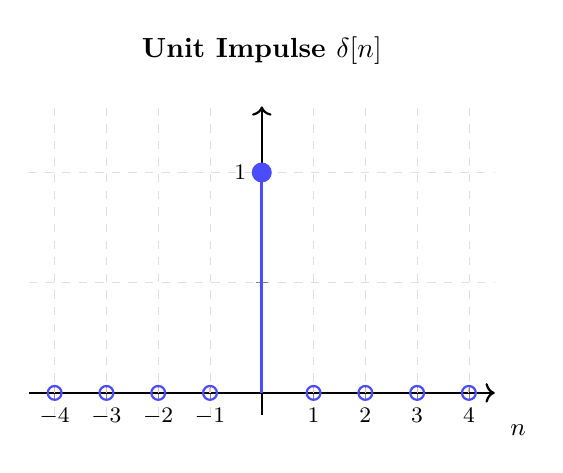
\begin{tikzpicture}
			\begin{axis}[
				width=7.5cm,
				height=5.5cm,
				axis lines=middle,
				xlabel={$n$},
				ylabel={},
				xmin=-4.5, 
				xmax=4.5,
				ymin=-0.1, 
				ymax=1.3,
				xtick={-4,-3,-2,-1,0,1,2,3,4},
				ytick={0,0.5,1},
				yticklabels={0,,1},
				grid=major,
				grid style={line width=0.2pt, draw=gray!25, dashed},
				font=\small,
				label style={font=\small},
				tick label style={font=\footnotesize},
				xlabel style={at={(axis description cs:1.05,0)}, anchor=north},
				ylabel style={at={(axis description cs:0,1.05)}, anchor=south},
				axis line style={->, thick},
				clip=false,
				title={Unit Impulse $\delta[n]$},
				title style={at={(0.5,1.05)}, font=\normalsize\bfseries}
				]
				% Plot the impulse at n=0 with stem
				\addplot[
				ycomb,
				very thick,
				color=blue!70,
				mark=*,
				mark size=3pt,
				mark options={fill=blue!70, draw=blue!70}
				] coordinates {(0,1)};
				% Add label for the impulse
				% Plot zeros with different style
				\addplot[
				only marks,
				mark=o,
				mark size=2.5pt,
				mark options={fill=blue, draw=blue!70, thick}
				] coordinates {(-4,0)(-3,0)(-2,0)(-1,0)(1,0)(2,0)(3,0)(4,0)};
				% Vertical lines for zeros (use \pgfplotsinvokeforeach)
				\pgfplotsinvokeforeach{-4,-3,-2,-1,1,2,3,4}{
					\draw[red!30, thin] (axis cs:#1,0) -- (axis cs:#1,0.02);
				}
			\end{axis}
		\end{tikzpicture}
		\caption{Unit Impulse}
	\end{subfigure}
	\hfill
	% Second subfigure: Unit Step
	\begin{subfigure}{0.48\textwidth}
		\centering
		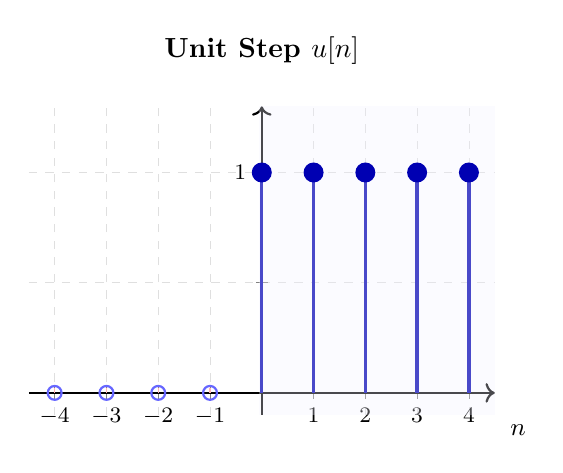
\begin{tikzpicture}
			\begin{axis}[
				width=7.5cm,
				height=5.5cm,
				axis lines=middle,
				xlabel={$n$},
				ylabel={},
				xmin=-4.5, 
				xmax=4.5,
				ymin=-0.1, 
				ymax=1.3,
				xtick={-4,-3,-2,-1,0,1,2,3,4},
				ytick={0,0.5,1},
				yticklabels={0,,1},
				grid=major,
				grid style={line width=0.2pt, draw=gray!25, dashed},
				font=\small,
				label style={font=\small},
				tick label style={font=\footnotesize},
				xlabel style={at={(axis description cs:1.05,0)}, anchor=north},
				ylabel style={at={(axis description cs:0,1.05)}, anchor=south},
				axis line style={->, thick},
				clip=false,
				title={Unit Step $u[n]$},
				title style={at={(0.5,1.05)}, font=\normalsize\bfseries}
				]
				% Plot ones (n >= 0) with stems
				\addplot[
				ycomb,
				very thick,
				color=blue!70!black,
				mark=*,
				mark size=3pt,
				mark options={fill=blue!70!black, draw=blue!70!black}
				] coordinates {(0,1)(1,1)(2,1)(3,1)(4,1)};
				% Labels for the ones
				% Plot zeros (n < 0)
				\addplot[
				only marks,
				mark=o,
				mark size=2.5pt,
				mark options={fill=blue, draw=blue!60, thick}
				] coordinates {(-4,0)(-3,0)(-2,0)(-1,0)};
				% Vertical lines for zeros
				\pgfplotsinvokeforeach{-4,-3,-2,-1}{
					\draw[red!30, thin] (axis cs:#1,0) -- (axis cs:#1,0.02);
				}
				% Background shading for n >= 0 region
				\fill[blue!5, opacity=0.3] (axis cs:-0.05,-0.1) rectangle (axis cs:4.5,1.3);
			\end{axis}
		\end{tikzpicture}
		\caption{Unit Step}
	\end{subfigure}

	\label{fig:discrete_signals}
\end{figure}

	\caption{Fundamental discrete-time signals}
		\label{fig:dt_impulse_and_step}
	\end{figure}
\newpage	
	\paragraph{Properties:}
	\begin{itemize}[noitemsep]
		\item The impulse is the first difference of the step:
		\[
		\imp[n] = u[n] - u[n-1].
		\]
	\end{itemize}
	
	% --- PLOT: Relation between DT step and impulse ---
	\begin{figure}[H]
		\centering
		\begin{figure}[H]
	\centering
	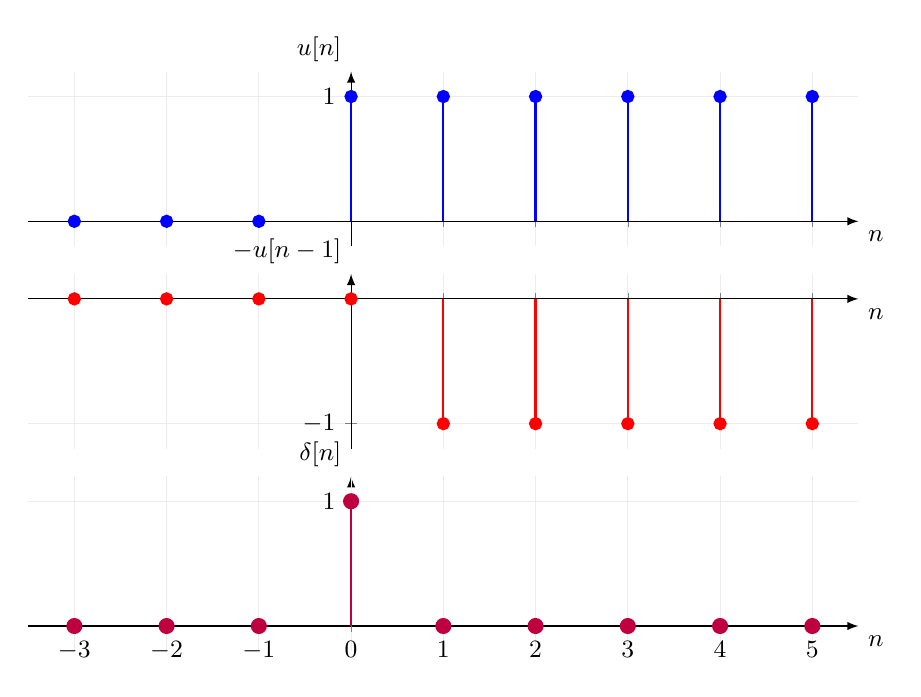
\begin{tikzpicture}
		\begin{groupplot}[
			group style={group size=1 by 3, vertical sep=10pt, xticklabels at=edge bottom},
			/tikz/font=\small,
			width=\linewidth, height=3.8cm, myaxes,
			xmin=-3.5, xmax=5.5,
			samples at={-3,...,5},
			xtick={-3,-2,-1,1,2,3,4,5}]
			
			\nextgroupplot[xlabel={$n$}, ylabel={$u[n]$}, ymin=-0.2, ymax=1.2, ytick={0,1}]
			\addplot[ycomb, mark=*, thick, blue] {(x>=0) ? 1 : 0};
			
			\nextgroupplot[xlabel={$n$}, ylabel={$-u[n-1]$}, ymin=-1.2, ymax=0.2, ytick={-1,0}]
			\addplot[ycomb, mark=*, thick, red] { -((x>=1) ? 1 : 0) };
			
			\nextgroupplot[xlabel={$n$}, ylabel={\(\delta[n]\)}, ymin=-0.2, ymax=1.2, ytick={0,1},
			extra x ticks={0}, extra x tick labels={0}]
			\addplot[ycomb, mark=*, thick, purple, mark size=2.5pt]
			{ ((x>=0) ? 1 : 0) - ((x>=1) ? 1 : 0) };
		\end{groupplot}
	\end{tikzpicture}
\end{figure}
		\caption{Relation between discrete-time step and impulse.}
		\label{fig:dt_step_impulse}
	\end{figure}
	
	\begin{itemize}[noitemsep]
		\item The step is the running sum of the impulse:
		\[
		u[n] = \sum_{k=-\infty}^n \imp[k] = \sum_{k=0}^\infty \imp[n-k].
		\]
		\item For any \(x[n]\): \(x[n] \imp[n - n_0] = x[n_0] \imp[n - n_0]\).
		\item The impulse is even:
		\[
		\imp[-n] = \imp[n].
		\]
	\end{itemize}
	\newpage
	\subsection*{Continuous-Time (CT) Signals}
	
	\paragraph{Unit Step \(u(t)\):}
	\[
	u(t) = \begin{cases}
		1, & t \geq 0 \\
		0, & t < 0
	\end{cases}
	\]
	
	% --- PLOT: CT Unit Step ---
	\begin{figure}[H]
		\centering
		\begin{figure}[H]
	\centering
	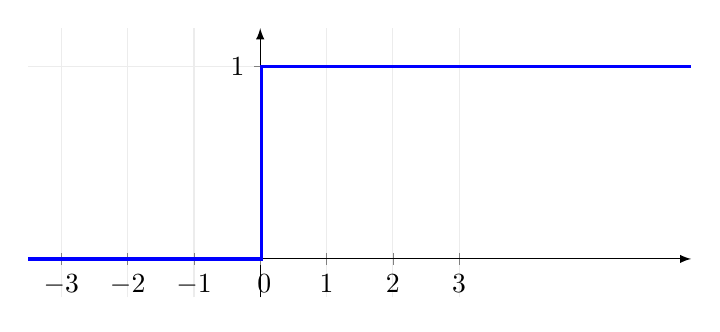
\begin{tikzpicture}
		\begin{axis}[
			myaxes,
			width=10cm, height=5cm,
			xmin=-3.5, xmax=6.5,
			ymin=-0.2, ymax=1.2,
			domain=-3.5:6.5, samples=200,
			ytick={1}, yticklabels={1},
			xtick={-3,-2,-1,1,2,3},
			extra x ticks={0},
			extra x tick labels={0},
			extra x tick style={grid=none, ticklabel style={xshift=1.5pt}},
			xlabel style={at={(axis description cs:1.03,0)}, anchor=south east}
			]
			\addplot[blue, very thick, const plot] { (x<0) ? 0 : 1 };
		\end{axis}
	\end{tikzpicture}
\end{figure}
		\caption{Continuous-time unit step function.}
		\label{fig:ct_unit_step}
	\end{figure}
	
	\paragraph{Unit Impulse \(\imp(t)\) (Dirac Delta Function):}
	The CT unit impulse is an idealized function defined by its properties under integration rather than its value. Conceptually, it is an infinitely tall, infinitely narrow pulse at \(t=0\) with a total area of 1.
	
	Formally, it can be viewed as the limit of a pulse \(g_T(t)\) shrinking in width but maintaining unit area:
	\[
	\imp(t) = \lim_{T \to 0} g_T(t).
	\]
	
	% --- PLOT: CT Impulse Approximation ---
	\begin{figure}[H]
		\centering
		\begin{figure}[H]
	\centering
	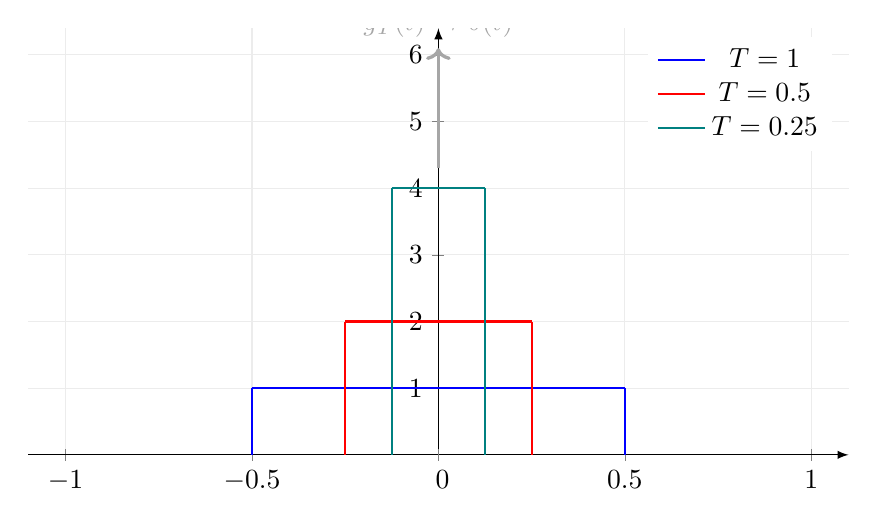
\begin{tikzpicture}
		\begin{axis}[
			myaxes,
			width=12cm, height=7cm,
			xmin=-1.1, xmax=1.1,
			ymin=0, ymax=6.4,
			xtick={-1,-0.5,0.5,1},
			extra x ticks={0},
			extra x tick labels={0},
			extra x tick style={grid=none, ticklabel style={xshift=1.5pt}},
			ytick={1,2,3,4,5,6},
			legend style={at={(0.98,0.98)}, anchor=north east, draw=none, fill=white},
			xlabel style={at={(axis description cs:1.03,0)}, anchor=south east}
			]
			
			\addplot[blue, thick, const plot, samples=2, domain=-0.5:0.5] {1};
			\addplot[blue, thick, forget plot] coordinates {(-0.5,0) (-0.5,1)};
			\addplot[blue, thick, forget plot] coordinates {(0.5,0) (0.5,1)};
			\addlegendentry{$T=1$}
			
			\addplot[red, thick, const plot, samples=2, domain=-0.25:0.25] {2};
			\addplot[red, thick, forget plot] coordinates {(-0.25,0) (-0.25,2)};
			\addplot[red, thick, forget plot] coordinates {(0.25,0) (0.25,2)};
			\addlegendentry{$T=0.5$}
			
			\addplot[teal, thick, const plot, samples=2, domain=-0.125:0.125] {4};
			\addplot[teal, thick, forget plot] coordinates {(-0.125,0) (-0.125,4)};
			\addplot[teal, thick, forget plot] coordinates {(0.125,0) (0.125,4)};
			\addlegendentry{$T=0.25$}
			
			\draw[gray!70, very thick, ->]
			(axis cs:0,4.3) -- (axis cs:0,6.1)
			node[above, align=center] {$T \downarrow 0$\\$g_T(t)\to \delta(t)$};
		\end{axis}
	\end{tikzpicture}
\end{figure}
		\caption{Continuous-time unit impulse approximation.}
		\label{fig:ct_impulse_approx}
	\end{figure}
	
	% --- PLOT: CT Impulse Representation ---
	\begin{figure}[H]
		\centering
		\begin{figure}[H]
	\centering
	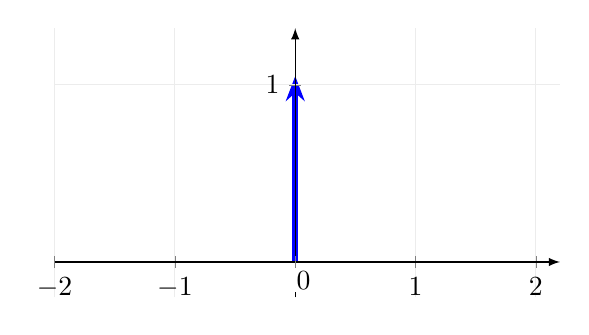
\begin{tikzpicture}
		\begin{axis}[
			myaxes,
			width=8cm, height=5cm,
			xmin=-2, xmax=2.2,
			ymin=-0.2, ymax=1.32,
			ytick={1}, yticklabels={1},
			xtick={-2,-1,1,2},
			extra x ticks={0},
			extra x tick labels={0},
			extra x tick style={grid=none, ticklabel style={xshift=3pt, fill=white, inner sep=1pt}},
			axis on top=true,
			xlabel style={at={(axis description cs:1.06,0)}, anchor=south east}
			]
			\draw[blue, line width=2.2pt] (axis cs:0,0) -- (axis cs:0,1);
			\draw[blue, line width=2.6pt, -{Stealth[length=9pt]}]
			(axis cs:0,1) -- (axis cs:0,1.05);
		\end{axis}
	\end{tikzpicture}
\end{figure}
		\caption{Continuous-time unit impulse representation.}
		\label{fig:ct_impulse}
	\end{figure}
	
	\paragraph{Properties:}
	\begin{itemize}[noitemsep]
		\item Sifting property: The impulse "sifts out" the value of a function at a single point:
		\[
		\int_{-\infty}^\infty x(t) \imp(t - t_0) \, \dt = x(t_0).
		\]
		\item The total area is unity:
		\[
		\int_{-\infty}^\infty \imp(t) \, \dt = 1.
		\]
		\item The impulse is the derivative of the step:
		\[
		\imp(t) = \frac{\dd}{\dd t} u(t),
		\]
		and the step is the integral of the impulse:
		\[
		u(t) = \int_{-\infty}^t \imp(\tau) \, \dd\tau.
		\]
		\item Scaling property:
		\[
		\imp(a t + b) = \frac{1}{|a|} \imp \left(t + \frac{b}{a} \right).
		\]
		\item The impulse is even:
		\[
		\imp(-t) = \imp(t).
		\]
	\end{itemize}
	
	\section*{Summary and Next Lecture}
	\begin{itemize}[noitemsep]
		\item Defined periodicity for CT and DT signals.
		\item Explored signal symmetries: even and odd decomposition.
		\item Introduced fundamental exponential and sinusoidal signals.
		\item Defined the unit impulse and unit step functions.
		\item \textbf{Next time:} System properties and classifications.
	\end{itemize}
	
\end{document}